\chapter*{Example chapter - remove}\label{chap:Example}

You can remove this chapter by deleteting the ``\texttt{\textbackslash include\{Chapter0\}}'' line in the \texttt{e344\_A1\_report.tex} file.  

\textcolor{red}{The document you submit must not have ANY red text in - the text in red in this template is for information only}. 
Introduce the reader to what you want to present in this chapter. 
Think carefully of what you want to convey. You want the reader (e.g. another student) to understand the main concepts -- they need to understand enough to safely and efficiently \textbf{use} and \textbf{design for} a chassis car, but abstract enough to not get caught up in the minutiae of electrons. The person assessing your report will consider whether you have demonstrated that you were able to find, integrate (absorb), and effectively convey knowledge on this topic.   So, write a short summary of information you gathered from literature (papers, web sites, datasheets). Include any references to literature you feel is needed. Be sure to cite all the references, which you can add in the \texttt{References.bib} file, using the \texttt{\textbackslash\{cite\}} command.\\

\noindent Some examples of how to cite (all of these have been added in the  \texttt{References.bib} file): 
It was stated by \cite{Booysen:2013} that ... . Subsequently, he changed his mind and said in  \cite{Gerber:2019} that ... .
While \cite{WebsiteOpAmp} claims it to be ... .
Figure \ref{fig:someName} shows a figure, which could paint a thousand words (if it does not, rather use words)! Table \ref{tab:PVresults} could capture some of your datasheet and/or measured results.

\begin{figure}[!htb]
\centering
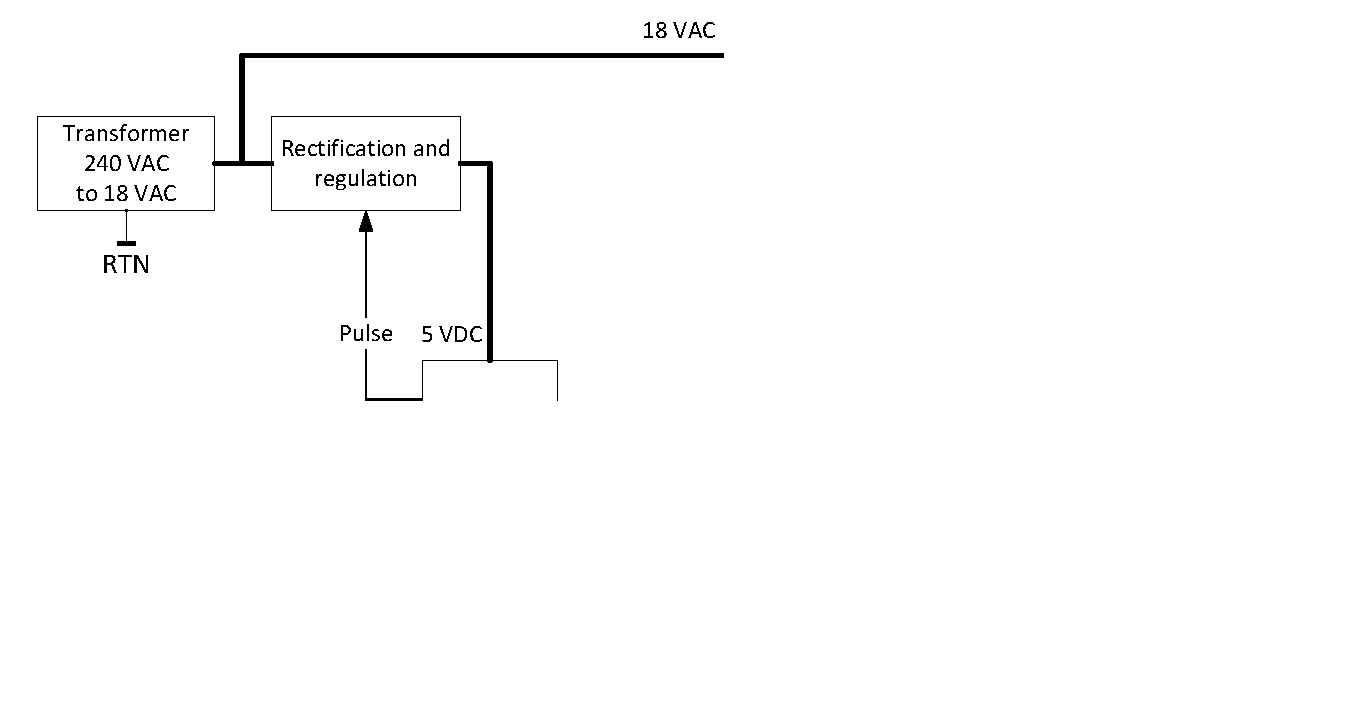
\includegraphics[width=0.5\linewidth]{Figures/PowerSystemDiagram.pdf}
\caption[This is my caption, make me descriptive!]{This is my caption, make me descriptive! And cite if you borrow figures \cite{WebsiteOpAmp}.}
\label{fig:someName}
\end{figure}

\begin{table}[!htb]
        \centering
        \footnotesize
        \caption{Example of a simple table.}
         \begin{tabular}{lrrrr}
          \toprule
             & $V_{OC}$ & $I_{CC}$ & $V_{pmax}$ \\
             &  [V]  & [A] & [V]\\
          \midrule
          Theroretical per cell & 1.0      & 1.0 & 1.0 \\
          Datasheet  per module &  1.0      & 1.0 & 1.0 \\
          Measured dark  1.0      & 1.0 & 1.0 \\
          Measured upside-down  1.0      & 1.0 & 1.0 \\
          Measured oblique  1.0      & 1.0 & 1.0 \\
          Measured facing  1.0      & 1.0 & 1.0 \\
          \bottomrule
        \end{tabular}
     \label{tab:PVresults}
\end{table}
